% Created 2017-04-15 Sat 11:00
% Intended LaTeX compiler: pdflatex
\documentclass[doctor,secret]{thuthesis}
\usepackage[utf8]{inputenc}
\usepackage[T1]{fontenc}
\usepackage{graphicx}
\usepackage{grffile}
\usepackage{longtable}
\usepackage{wrapfig}
\usepackage{rotating}
\usepackage[normalem]{ulem}
\usepackage{amsmath}
\usepackage{textcomp}
\usepackage{amssymb}
\usepackage{capt-of}
\usepackage{hyperref}
\usepackage[myhdr]{commons}
\usepackage{thuthesis}
\usepackage{hyperref}
\graphicspath{{figures/}}
\author{Daniel}
\date{\today}
\title{}
\hypersetup{
 pdfauthor={Daniel},
 pdftitle={},
 pdfkeywords={},
 pdfsubject={},
 pdfcreator={Emacs 25.2.1 (Org mode 9.0.5)}, 
 pdflang={English}}
\begin{document}

\thusetup{
%******************************
% 注意:
%   1. 配置里面不要出现空行
%   2. 不需要的配置信息可以删除
%******************************
%
%=====
% 秘级
%=====
secretlevel={秘密},
secretyear={10},
%
%=========
% 中文信息
%=========
ctitle={智慧医院的设计与实现-以宜昌市第一人民医院为例},
cdegree={管理学硕士},
cdepartment={水利与环境学院},
cmajor={项目管理},
cauthor={吴为民},
csupervisor={郑霞忠教授},
% cassosupervisor={陈文光教授}, % 副指导老师
% ccosupervisor={某某某教授}, % 联合指导老师
% 日期自动使用当前时间,若需指定按如下方式修改:
% cdate={超新星纪元},
%
% 博士后专有部分
% cfirstdiscipline={计算机科学与技术},
% cseconddiscipline={系统结构},
% postdoctordate={2009 年 7 月——2011 年 7 月},
% id={编号}, % 可以留空:id={},
% udc={UDC}, % 可以留空
% catalognumber={分类号}, % 可以留空
%
%=========
% 英文信息
%=========
etitle={Design and Application of Smart Medical Service },
% 这块比较复杂,需要分情况讨论:
% 1. 学术型硕士
%    edegree:必须为 Master of Arts 或 Master of Science(注意大小写)
%             “哲学、文学、历史学、法学、教育学、艺术学门类,公共管理学科
%              填写 Master of Arts,其它填写 Master of Science”
%    emajor:“获得一级学科授权的学科填写一级学科名称,其它填写二级学科名称”
% 2. 专业型硕士
%    edegree:“填写专业学位英文名称全称”
%    emajor:“工程硕士填写工程领域,其它专业学位不填写此项”
% 3. 学术型博士
%    edegree:Doctor of Philosophy(注意大小写)
%    emajor:“获得一级学科授权的学科填写一级学科名称,其它填写二级学科名称”
% 4. 专业型博士
%    edegree:“填写专业学位英文名称全称”
%    emajor:不填写此项
edegree={Master of Science},
emajor={Engineering Project Management},
eauthor={Wu Weimin},
esupervisor={Professor Zheng Xiazhong},
% eassosupervisor={Chen Wenguang},
% 日期自动生成,若需指定按如下方式修改:
% edate={December, 2005}
%
% 关键词用“英文逗号”分割
ckeywords={信息化, 智慧医院,架构, 设计},
ekeywords={Informationalism, Smart Hospital, Architecture, Design}
}

% 定义中英文摘要和关键字
\begin{cabstract}
近年来,随着智能终端技术、物联网技术、互联网技术的不断发展和融合,这些新技术在家居生活、交通运输、农业生产、工业生产、医疗卫生等领域得到了越来越广泛的应用,使得人们的工作和生活变得越来越舒适便捷。但就目前而言,新技术在医疗卫生行业的应用仍有很大发展空间,尤其是在医院信息化建设和看病难的背景下,传统的护士站、医生站等固定信息点的功能已无法满足人们日益增长的需求。因此,如何引入这些新技术,设计一套实用性强、成本低廉的智能医疗信息管理系统,以实现人们的轻松就医和医护人员的高效管理,成为了需要迫切研究的课题。针对当前医院信息管理的问题和不足,本文融合物联网等技术,开发了一套智慧医院信息控制系统。使用该系统,就诊者能够通过 Android 手机客户端轻松便捷地进行预约挂号、查看诊疗记录和医院新闻动态等;医护人员能够通过 WEB 信息管理平台更方便地完成本职工作和各项信息指标的查看,更全面的实现医院的管理。本文主要在应用层对基于物联网的智慧医院信息控制系统进行了研究,研究主要包括 Android 客户端和 WEB 管理平台两部分的内容:(1)Android 客户端采用 Eclipse 平台进行开发,应用了 MVC 开发模式和模块化设计的编程思想。Android 客户端服务于就诊者,与 WEB 平台服务器通过 HTTP 协议进行通讯,实现数据共享。用户在使用客户端时必须先进行账号注册和登录校验,保证了患者的医疗隐私安全。其个人信息管理模块提供个人信息修改和附加、切换就诊者功能,实现一个账号多人就医,适合家庭使用。(2)WEB 管理平台采用 JavaWeb 技术进行编写,应用了 MySql 数据库进行数据存储。在管理平台内进行权限区分,使平台同时面向门诊部、护士站、住院部和医院管理员。平台通过 Socket 协议与下层网关相连,获取病房环境信息,下发电器控制指令。综上,本文研究的基于物联网的智慧医院信息控制系统为就诊者、医生、护士、医院管理员等多种用户人群提供服务,既方便了患者就医,又方便了医护人员工作和医院的综合管理,对改善我国就医难问题和推进我国医院信息化建设有着重要的意义
本文的创新点主要有:
\begin{itemize}
\item 智慧医院信息化流程的改进;
\item 电子病历体系的设计;
\end{itemize}


\end{cabstract}

% 如果习惯关键字跟在摘要文字后面,可以用直接命令来设置,如下:
% \ckeywords{\TeX, \LaTeX, CJK, 模板, 论文}

\begin{eabstract}

\end{eabstract}

% \ekeywords{\TeX, \LaTeX, CJK, template, thesis}
\makecover
%% 目录
\tableofcontents

%% 符号对照表
%%\input{data/denotation}

%%% 正文部分
\mainmatter
%%%\include{data/chap01}
%%%\include{data/chap02}
\chapter{绪论}
\label{sec:org2a308e2}
现代社会,人口快速增长、老龄化趋势不断加快、生态环境恶化、自然事故频发,同时人们自我健康意识不断增强,多方面因素让我们对医疗卫生保障体系提出了更高的建设要求。我们需要利用通信和信息技术手段不断提高医院的运营和管理效率、降低医院经营成本,从而满足人们健康生活的基本愿望,促进社会稳定发展 \cite{__2011,__2011-1,__2016-11,__2016-10}。

信息化技术在解决人比较集中,人力成本比较高的领域具有独特的效果。医院在现代社会是一个人流高度集中,工作流程相对复杂的信息化领域。在国内的医疗行业中,信息化建设由于新的技术影响,发展很迅速,各区域医疗服务均借助于云计算、物联网、大数据等新技术推动新一轮的医疗体制改革,其成果可能改变中国的医疗运作模式 \cite{__2016-6,__2016-5,__2016-4,__2016-3,__2015-21,__2015-20,__2015-19,__2015-18}。
\section{智慧医院起源}
\label{sec:org37bf885}
“智慧医疗” \cite{__2012,__2016-4,__2013-2} 源自 IBM 于 2008 年提出的“智慧地球”概念,旨在利用先进的互联网及信息化技术来改善疾病预防、诊断和研究,并最终让医疗生态圈的各个组成全部受益。在理想的智慧医疗体系中,有居民个人健康档案区域医疗信息平台,并利用最先进的物联网技术,实现患者与医务人员、医疗机构、医疗设备之间的互动。智慧医疗由三部分组成,分别为智慧医院系统、区域卫生系统以及家庭健康。

传统的数字化医院指利用计算机和数字通信网络等信息技术,实现语音、图像、文字、数据、图表等信息的数字化采集、存储、阅读、复制、处理、检索和传输。数字化医疗设备系统主要包括:医院信息系统(即 Hospital Information System ,HIS)、医学影像和通信系统(Picture Archiving and Communication Systems,PACS)和办公自动化系统(Office Automation,OA)。其主要特征:无纸化、无胶片化、无线网络化。

智慧医院是数字化医院发展的新阶段,是基于计算机网络技术发展,应用计算机、通讯、多媒体、网络等其他信息技术,突破传统医学模式中时空限制,实现疾病的预防、保健、诊疗、护理等业务管理和行政管理自动化数字化运作。在全部医疗流程中实现全面的数字化、涵盖了联机业务处理系统(On-Line Transaction Processing,OLTP)、医院信息系统(HIS)、临床信息系统(ClimcalInfoimation system,CIS)、,互联网系统(Intranet/Internet)、远程医学系统(Tele medicine)、智能楼宇管理系统。其特征:全网络化。

智慧医院的核心理念是“以患者为中心”,利用各种信息化手段方便患者就医、简化就医流程,降低就医成本,最终实现患者自助就医。在智慧医院的每个工作环节中,都应尽可能以信息技术为基础,同时管理制度及医院文化等方面也应与硬件基础数字化整合,实现软硬件的有机结合。智慧医院最大的特征在于具备主动感知和智能调控能力,能够更好地为医务人员和病患服务。

\section{智慧医院解决患者痛点}
\label{sec:org5f8c752}
智慧医院在原有的数字医院的基础上,通过对医院信息系统(HIS)、实验室信息管理系统(Laboratory Information Management System,LIS)、医学影像信息的存储系统(PACS)和传输系统以及医生工作站四个部分信息整合,实现病人诊疗信息和行政管理信息的收集、存储、处理、提取及数据交换。同时,创新性地以现代智能移动终端为切入点,让患者能够更多地参与到诊疗过程当中,实现从诊前到诊后的“一站式”服务。

传统医院中,患者抱怨最多问题往往是:“三长”即挂号候诊时间长、取检查报告时间长、缴费报账时间长。在智慧医院体系中,“三长”问题得到了根本性缓解。

诊前服务:主要包括在线智能分诊、在线预约挂号、诊前叫号查询和医院信息查询等功能。患者登陆医院网站或打开掌上医院 APP,选择性别、年龄,然后根据人体模型选择不舒服的部位,比如,咳嗽可以点“胸部”,系统就显示出脓痰、干咳、咳痰等主要症状和伴随症状,并显示可能性疾病,推荐病人到相应的科室挂号。同时,患者还能快速方便的查询到各类健康资讯,以及医院、科室和医生的全方面信息,方便患者选择。

诊中服务:利用掌上医院 APP、微信或支付宝服务窗等,用户可以轻松实现移动端缴费、查询报告单等功能。以往,患者为取检查检验报告单需要等候数小时,甚至数天时间,无形中增加了患者看病的时间和金钱成本。现在,患者绑定就诊信息后可以直接在掌上医院 APP 或微信支付宝服务窗中查询各类检查检验结果。部分智慧医院甚至提供了患者诊后直接在 APP 上与医生沟通的功能,进一步减少患者不必要的奔波。同时,医生可以直接将各类预先整理好的疾病健康宣教资料推送给患者,提高了医患沟通的效率。

诊后服务:在我国,由于医疗资源分布不均衡和医院间患者信息交流不畅,造成了大型医院人满为患,小型医疗机构无人问津的局面。同时患者如果想知道自己的历史就医记录,除了翻阅一本又一本纸质的病历外,根本无从查阅。智慧医院的出现让患者可以通过手机应用查看个人曾在医院的历史预约和就诊记录,包括门诊或住院病历、用药历史、治疗情况、相关费用、检查单检验单图文报告、在线问诊记录等,不仅可以及时自查健康状况,还可通过 24 小时在线医生进行咨询。在健全个人电子健康档案的基础上,部分智慧医院利用区域医疗平台,可以实现远程会诊,双向转诊等功能。同时,通过整合各类智能终端设备,远程监测患者生理体征,实现慢病管理智能化。

本论文研究智慧医院解决方案,有效的降低了医院运营的成本、减少了医疗差错发生的概率、提高了管理者的监管水平、改善了病人的服务体验、实现了医院内部办公的无纸化、无胶片化、无线化、营造了绿色的工作环境。

智慧医院解决方案,覆盖了从医院管理和临床的信息化到相关基础设施(网络、数据中心等)的建设。针对医院不同的应用场景,通过构建以电子病历为核心的医院综合信息平台,提供了移动医疗,远程医疗,基层医疗信息化,慢病管理,综合医疗云等智慧医院解决方案,服务 于医疗卫生行业。

\section{课题研究背景概述}
\label{sec:org30526b5}
过去的二十年,医院信息化在经历了以行政管理为中心、以医生诊疗为中心的初期发展阶段后,步入了以服务患者为中心的数字化医院发展阶段(如图\ref{fig:medicalinformationstages})。智慧医院以数字化医院建设为基础,需要实现包括网络服务、移动医疗、远程医疗、健康管理等服务于医疗患者的医疗业务新应用,然而新业务的运用让我们不得不面临着众多医院信息化的难题:
\begin{enumerate}
\item 门诊、住院、检验检查、科研、办公、院外等不同层面的多种重要信息系统并存,它们之间不互通、不兼容,也很难实现沟通 协同和统一管理,医院需要整合医疗信息系统,以便全面、直观的掌握医院经营状态;
\item 整个医院信息化资源需要统一经营,实现资源高效利用、新业务开展、节能、安全管控、降成本等综合经营目标;
\item 基层医疗机构缺乏信息化支持,需要实现医疗普及及医疗服务的一致性;
\item 解决慢病病人在医院外的健康管理,把业务推进到社区及家庭;
\item 医疗资源主要分布在大城市大医院,医疗资源分布的不均衡。
\end{enumerate}

\begin{figure}[htbp]
\centering
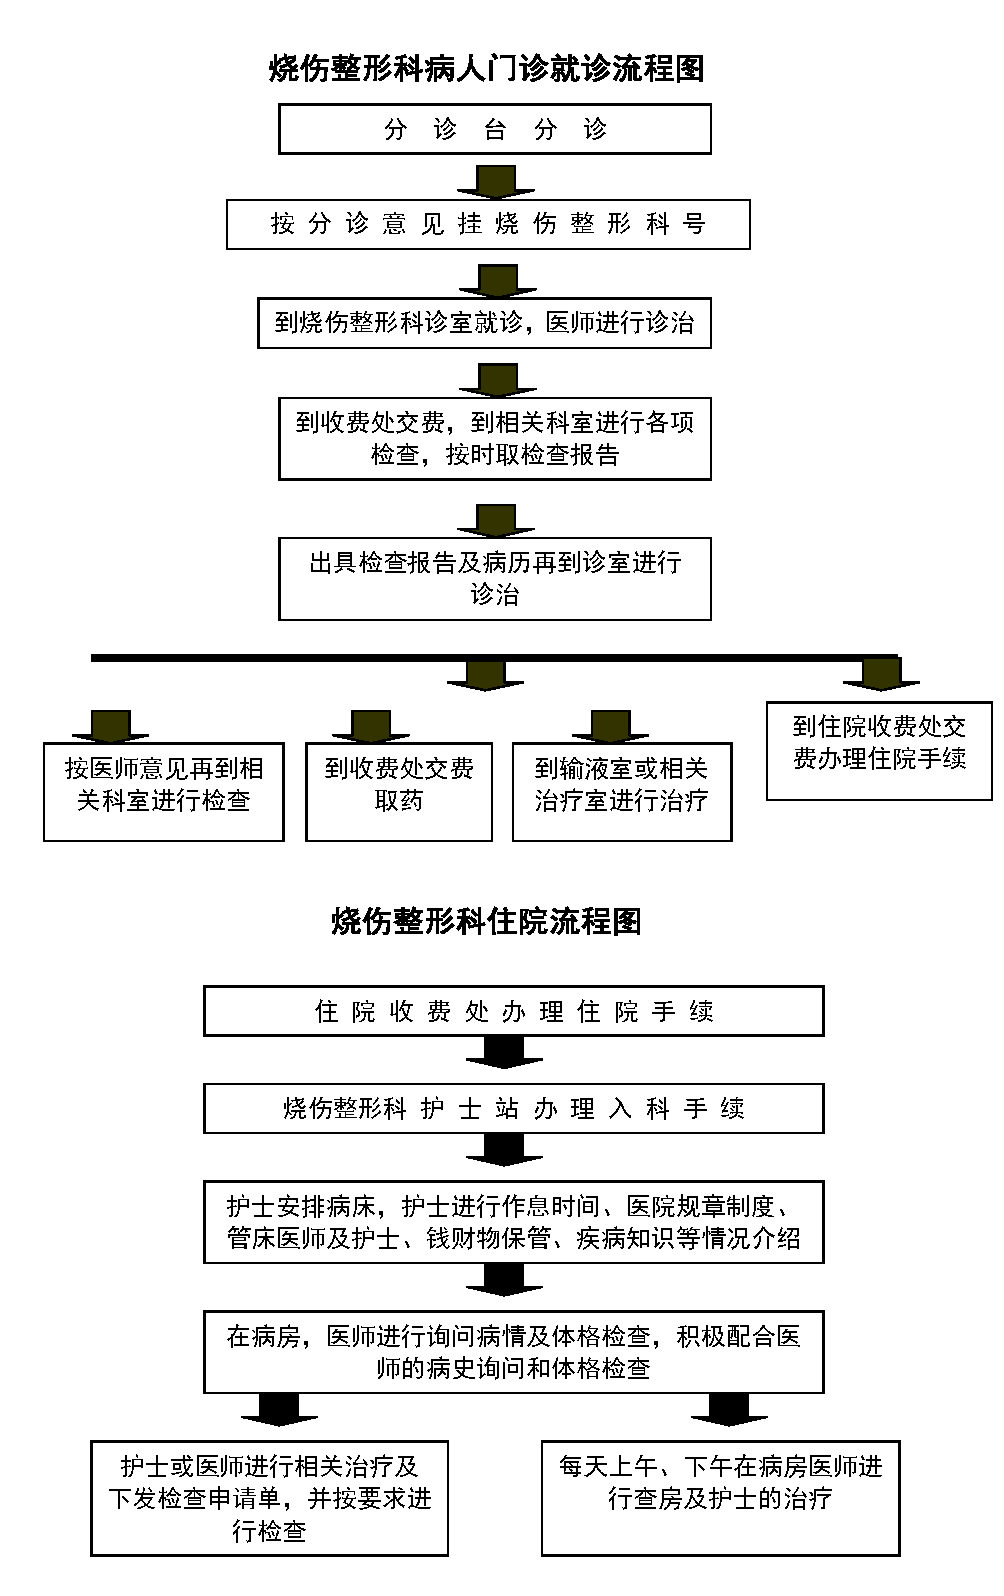
\includegraphics[width=0.8\textwidth]{figures/medicalinformationstags.pdf}
\caption{医院信息化发展的三个阶段 \label{fig:medicalinformationstages}}
\end{figure} 

现代化的医院信息化要求智慧医院解决方案同时考虑三个层面的问题:第一层面,医疗业务的信息化,实现网络化、无纸化、无胶片办公;第二层面,信息资源的管理,实现信息的整合、应用的整合,发挥信息化的优势;第三层面,从服务出发,激活医疗信息化的需求,激活时空阻隔,信息充分流通共享,持续创新,满足医疗服务的不断发展。

\section{课题研究意义及研究目标}
\label{sec:org4774b55}
本项目借助目前已经部分实现的宜昌智慧医疗系统,以及在宜昌市第一人民医院的应用实践,发现智慧医疗应用在实际医疗治理中存在的问题而提出。并基于以下基本出发点:
(1)	从患者角度出发
智慧医疗的核心就是“以患者为中心”,给予患者以全面、专业、个性化的医疗体验。
通过智慧医疗的整合区域医疗体系能够使大量的医疗监护工作实施网络化、无线化的应用,实现医疗信息的共享。如:社区医院可以预约三级医院的专家号和特殊检查,各种检查和检验结果各级医院共享共认,区域医疗“一卡通”等便民诊疗措施。
(2)	从医护等工作人员角度出发
智慧医疗通过快捷完善的数字化信息系统信使医护工作实现“无纸化、智能化、高效化”。不仅减轻了医护人员的工作强度,而且提升了诊疗速度,还让诊疗更加精准。在提高诊疗效率的同时也提高了医护人员的绩效,从而调动了医护人员的工作积极性。
(3)	从医疗机构的角度出发
整合的智慧医疗体系除去了医疗服务当中各种重复环节,降低了医院运营成本的同时也提高了运营效率和监管效率。
本项目研究智慧医疗与医疗治理之间的关系,通过实施智慧医疗的解决方案,研究实施医疗改革,医疗治理的技术路线,期望解决医疗资源分配不合理的矛盾,通过良好的信息沟通,全寿命周期的医疗信息跟踪,从根本上解决医患冲突和医患矛盾。在此基础上,进行医疗体制改革,尽管构建富有效率的医疗卫生体制是一个世界性的难题,纵观各国医疗卫生体制改革之路可以看出,尽管改革思路和方法有所不同,但在通过信息化手段全面构建并应用数字卫生系统,推动医疗卫生体制改革,更好地解决医疗卫生服务需求与服务供给的平衡方面都有着共同的期望。 
在国家新医改方案的统一指导下,通过智慧医疗,实现居民获得可及优质的卫生服务、连续的健康信息和全程健康管理;卫生服务机构保证服务质量,提高服务效率;公共卫生专业机构有效地开展疾病管理、卫生管理、应急管理、健康教育等工作;卫生行政部门提高卫生服务质量、强化绩效考核以及加强监管能力;医保、药监、计生、公安、民政等部门协同开展工作。
通过信息交换平台,提供对于疾病数据接近实时的访问。通过这些数据,提高医疗机构的医疗水平,起到良好的品牌效应,也能使用户能够预测和分析健康风险,为医院和国家腾出更多的时间用于准备可能出现的灾难性疾病爆发。
通过这一整合的医疗信息系统医院可对其就诊量、医生用药及检查检验情况、医保基金使用、财务结余等等业务运作的每一项数据都能做到实时监控。在最难把控的药品监管方面系统能从入库、每个医生工作站的使用、库存量、过期期限等全程跟踪每一种药品,使限制大处方、滥检查的实时监控成为现实。

\section{论文的组织结构}
\label{sec:org0d7967c}
\chapter{相关技术}
\label{sec:orgb6343b8}
\section{物联网技术}
\label{sec:org96d2e9a}
物联网技术的定义是:通过射频识别(RFID)、红外感应器、全球定位系统、激光扫描器等信息传感设备,按约定的协议,将任何物品与互联网相连接,进行信息交换和通讯,以实现智能化识别、定位、追踪、监控和管理的一种网络技术。
“物联网技术”的核心和基础仍然是“互联网技术”,是在互联网技术基础上的延伸和扩展的一种网络技术,其用户端延伸和扩展到了任何物品和物品之间,进行信息交换和通讯。
\href{figures/internetofthings.pdf}{internetthings}

物联网的主要技术支撑主要包含:
\begin{enumerate}
\item RFID: 电子标签属于智能卡的一类,物联网概念是 1999 年 MIT Auto-ID 中心主任 Ashton 教授提出来的,RFID 技术在物联网中主要起“使能”(Enable)作用;
\end{enumerate}
2.传感网:借助于各种传感器,探测和集成包括温度、湿度、压力、速度等物质现象的网络,也是温总理“感知中国”提法的主要依据之一;
\begin{enumerate}
\item M2M:这个词国外用得较多,侧重于末端设备的互联和集控管理,X-Internet,中国三大通讯营运商在推 M2M 这个理念;
\item 两化融合:工业信息化也是物联网产业主要推动力之一,自动化和控制行业是主力,但来自这个行业的声音相对较少。
\end{enumerate}
\section{快速原型编程}
\label{sec:orgd1e455e}
原型是指模拟某种产品的原始模型,在其他产业中经常使用。软件开发中的原型是软件的一个早期可运行的版本,它反映了最终系统的重要特性。
快速原型模型又称原型模型,它是增量模型的另一种形式;它是在开发真实系统之前,构造一个原型,在该原型的基础上,逐渐完成整个系统的开发工作。例如,客户需要一个 ATM 机软件,可以先设计一个仅包含刷卡、密码检测、数据输入和账单打印的原型软件提供给客户,此时还不包括网络处理与数据库存取以及数据应急、故障处理等服务。快速原型模型的第一步是建造一个快速原型,实现客户或未来的用户与系统的交互,用户或客户对原型进行评价,进一步细化待开发软件的需求。通过逐步调整原型使其满足客户的要求,开发人员可以确定客户的真正需求是什么;第二步则在第一步的基础上开发客户满意的软件产品.
\section{大数据技术}
\label{sec:org49fc1d4}
大数据(Big data),指的是传统数据处理应用软件不足以处理它们的大或复杂的数据集的术语[4][5]。在总数据量相同的情况下,与个别分析独立的小型数据集(Data set)相比,将各个小型数据集合并后进行分析可得出许多额外的信息和数据关系性,可用来察觉商业趋势、判定研究质量、避免疾病扩散、打击犯罪或测定即时交通路况等;这样的用途正是大型数据集盛行的原因[6][7][8]。
截至 2012 年,技术上可在合理时间内分析处理的数据集大小单位为艾字节(exabytes)[9]。在许多领域,由于数据集过度庞大,科学家经常在分析处理上遭遇限制和阻碍;这些领域包括气象学、基因组学[10]、神经网络体学、复杂的物理模拟[11],以及生物和环境研究[12]。这样的限制也对网络搜索、金融与经济信息学造成影响。数据集大小增长的部分原因来自于信息持续从各种来源被广泛收集,这些来源包括搭载感测设备的移动设备、高空感测科技(遥感)、软件记录、相机、麦克风、无线射频辨识(RFID)和无线感测网络。自 1980 年代起,现代科技可存储数据的容量每 40 个月即增加一倍[13];截至 2012 年,全世界每天产生 2.5 艾字节(2.5×1018 字节)的数据[14]。
大数据几乎无法使用大多数的数据库管理系统处理,而必须使用“在数十、数百甚至数千台服务器上同时平行运行的软件”(计算机集群是其中一种常用方式)[15]。大数据的定义取决于持有数据组的机构之能力,以及其平常用来处理分析数据的软件之能力。“对某些组织来说,第一次面对数百 GB 的数据集可能让他们需要重新思考数据管理的选项。对于其他组织来说,数据集可能需要达到数十或数百 TB 才会对他们造成困扰。”[16]
随着大数据被越来越多的提及,有些人惊呼大数据时代已经到来了,2012 年《纽约时报》的一篇专栏中写到,“大数据”时代已经降临,在商业、经济及其他领域中,决策将日益基于数据和分析而作出,而并非基于经验和直觉。但是并不是所有人都对大数据感兴趣,有些人甚至认为这是商学院或咨询公司用来哗众取宠的 buzzword,看起来很新颖,但只是把传统重新包装,之前在学术研究或者政策决策中也有海量数据的支撑,大数据并不是一件新兴事物。
大数据时代的来临带来无数的机遇,但是与此同时个人或机构的隐私权也极有可能受到冲击,大数据包含各种个人信息数据,现有的隐私保护法律或政策无力解决这些新出现的问题。有人提出,大数据时代,个人是否拥有“被遗忘权”,被遗忘权即是否有权利要求数据商不保留自己的某些信息,大数据时代信息为某些互联网巨头所控制,但是数据商收集任何数据未必都获得用户的许可,其对数据的控制权不具有合法性。2014 年 5 月 13 日欧盟法院就“被遗忘权”(right to be forgotten)一案作出裁定,判决谷歌应根据用户请求删除不完整的、无关紧要的、不相关的数据以保证数据不出现在搜索结果中。这说明在大数据时代,加强对用户个人权利的尊重才是时势所趋的潮流。
\section{机器学习技术}
\label{sec:orgb4ba571}
机器学习有下面几种定义: “机器学习是一门人工智能的科学,该领域的主要研究对象是人工智能,特别是如何在经验学习中改善具体算法的性能”\cite{enbom_should_2013}。 “机器学习是对能通过经验自动改进的计算机算法的研究”。 “机器学习是用数据或以往的经验,以此优化计算机程序的性能标准。” 一种经常引用的英文定义是:A computer program is said to learn from experience E with respect to some class of tasks T and performance measure P, if its performance at tasks in T, as measured by P, improves with experience E. 
机器学习已经有了十分广泛的应用,例如:数据挖掘、计算机视觉、自然语言处理、生物特征识别、搜索引擎、医学诊断、检测信用卡欺诈、证券市场分析、DNA 序列测序、语音和手写识别、战略游戏和机器人运用。\cite{tierney-gumaer_review_2006} 
\section{WSDL 技术}
\label{sec:org0e30ceb}
\section{MVC 设计模式}
\label{sec:orgeaf2a3a}
通常情况下,应用系统都具有界面显示、界面交互、数据处理、逻辑运算、数据存储、 通信等功能,每一种功能的实现都需要程序的支撑,且各具特色,各项功能之间也存在着 一些关联,因此,如何对应用程序进行层次划分,降低程序的耦合度,成为十分重要的问题,MVC 设计模式可以很好地解决这个问题。
MVC 是 Model View Controller 的简写,即模型-视图-控制器,是软件设计中经常采用的一种设计模式,该设计模式根据功能对各种对象(多指用以维护、表现数据的对象) 进行分割,及大地降低了程序的耦合度,提高了程序的重用性和可维护性。
目前,MVC 是一种非常流行的软件设计模式,具有分析方法更简便、设计框架和设计规范更清晰的特点,能够更好地帮助开发者理解和分析应用模型,开发者根据 MVC 设计模式按照模型、视图、控制器的方式将应用程序的输入、处理、输出强制分离,每个 模块担负着不同的任务,如图

1、控制器:指应用程序的行为,将来自用户的请求进行解释,映射为某种行为,交由模型负责实现,再选择视图显示执行结果。对于 Android 客户端来说,用户请求可能是按钮 点击等操作,对于 Web 平台来说则可能是按钮点击或客户端的 HTTP 请求。
2、模型:模型通常代表应用程序中的业务数据以及业务规则(business rule)。一个模型 可以被多个视图使用,极大提高了程序的重用性。
3、视图:视图是用户看到并与之交互的界面,负责向用户展示数据并采集用户在界面的 操作(点击、输入等),将用户操作请求发给控制器处理。此外,视图还可接收模型发出 的更新数据的通知,实现信息的同步更新。
\section{开发框架模型}
\label{sec:org1c47e72}
本项目使用开源的 spring 框架实现,采用 JEECG 轻量级开发框架实现,JEECG 是一款基于代码生成器的 J2EE 快速开发平台,开源界“小普元”超越传统商业企业级开发平台。引领新的开发模式(Online Coding 模式(自定义表单); 代码生成器模式; 手工 MERGE 智能开发), 可以帮助解决 Java 项目 60\%的重复工作,让开发更多关注业务逻辑。既能快速提高开发效率,节省人力成本,同时又不失灵活性。具备:表单配置能力(无需编码)、移动配置能力、工作流配置能力、报表配置能力(支持移动端)、插件开发能力(可插拔).采用 SpringMVC + Hibernate + Minidao(类 Mybatis) + Easyui(UI 库)+ Jquery + Boostrap + Ehcache + Redis + Ztree 等基础架构,采用面向声明的开发模式, 基于泛型编写极少代码即可实现复杂的数据展示、数据编辑、 表单处理等功能,再配合 Online Coding 在线开发与代码生成器的使用,将 J2EE 的开发效率提高 6 倍以上,可以将代码减少 80\%以上。
\chapter{需求分析与总体设计}
\label{sec:orge614e56}
\section{系统功能分析}
\label{sec:org9881e58}
解决方案总体布局如图\ref{fig:generalscheme}

\begin{figure}[htbp]
\centering
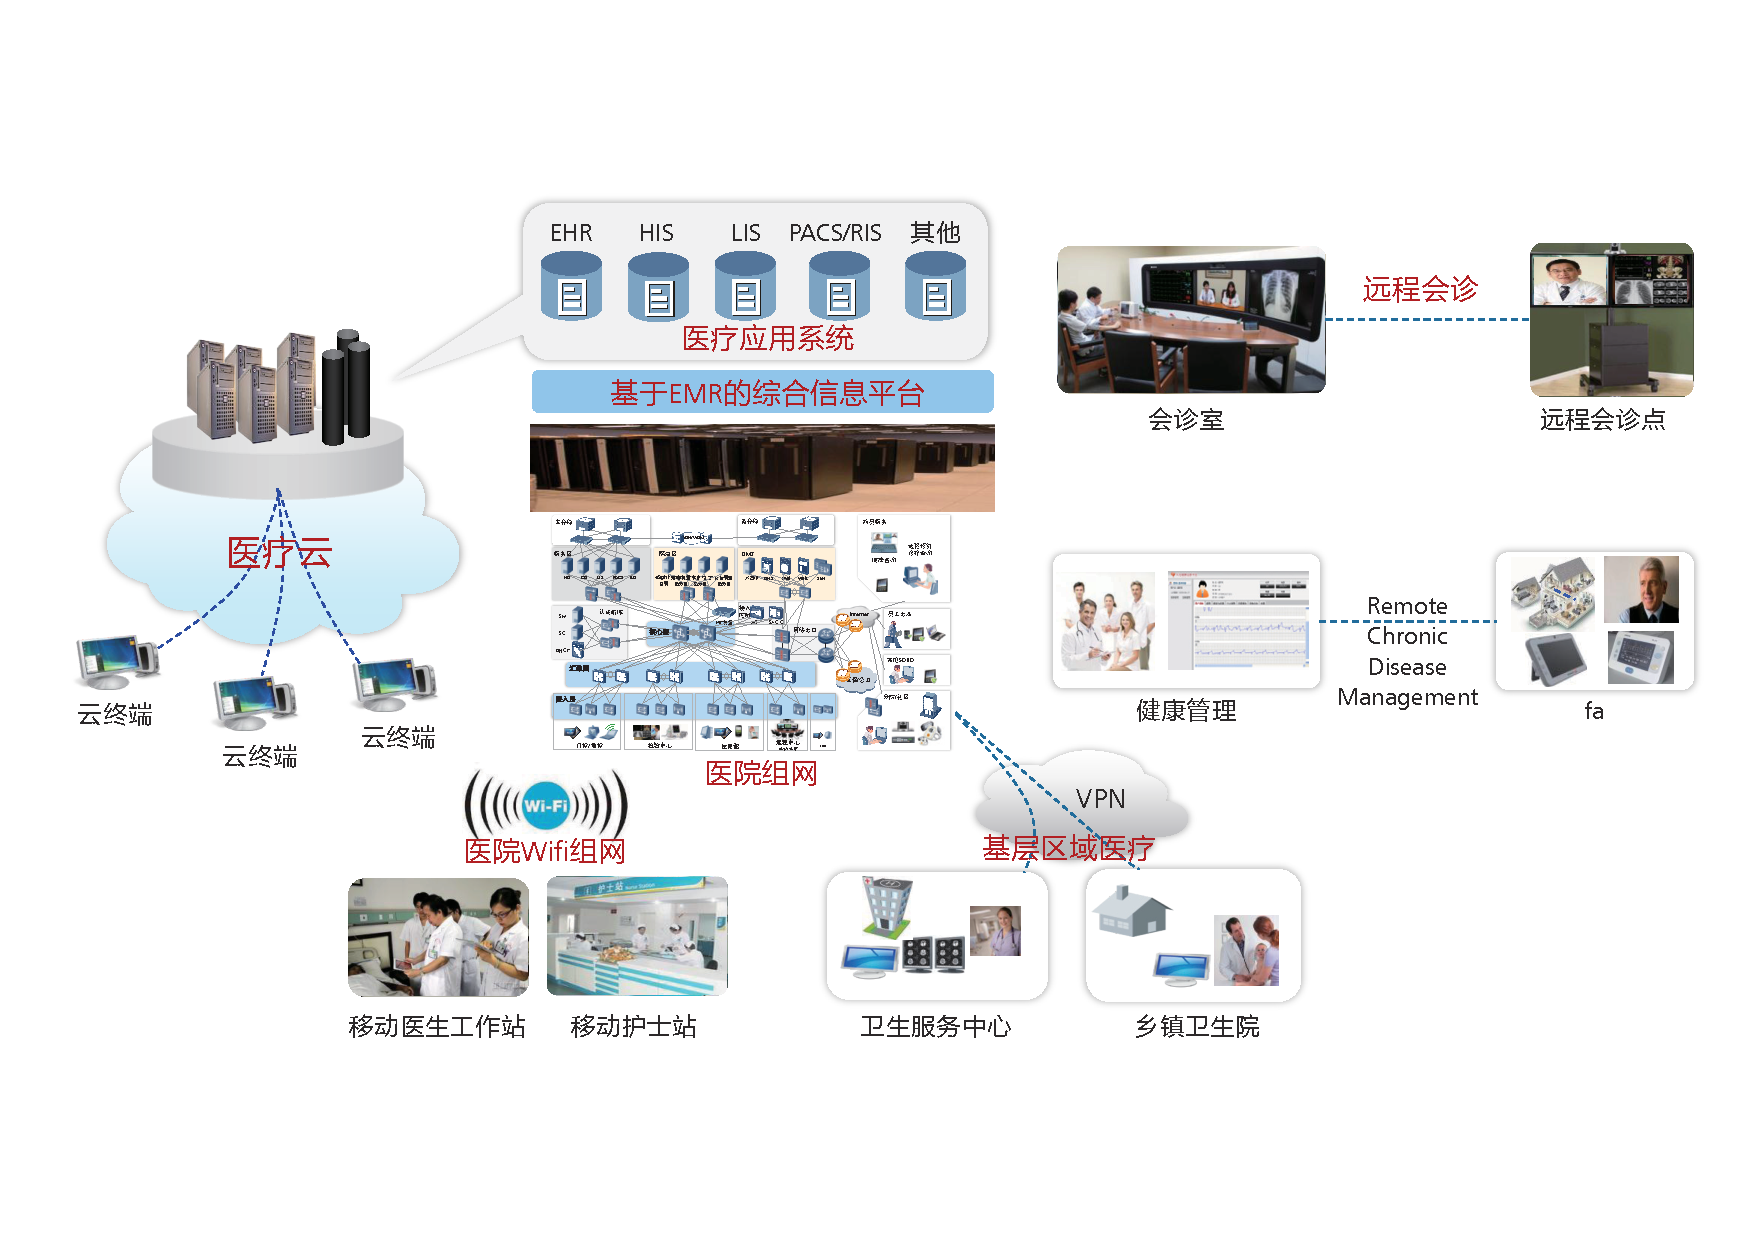
\includegraphics[width=0.8\textwidth]{figures/general-framework.pdf}
\caption{解决方案的整体架构 \label{fig:generalscheme}}
\end{figure} 

\subsection{预约挂号设计}
\label{sec:orgb71e788}
\subsection{诊疗模块}
\label{sec:orga3f3817}
\subsection{收费和消费模块}
\label{sec:org7c2a574}
\subsection{电子病历设计}
\label{sec:org189c068}
\section{智慧医院设计}
\label{sec:orgafa0baf}
\subsection{对象持久化设计}
\label{sec:org1ba75b3}
\subsection{前端设计}
\label{sec:org4a6fe2d}
\subsection{业务处理逻辑设计}
\label{sec:org5f05dca}
\section{网络架构的设计}
\label{sec:org18e5bc2}
网络结构设计如\ref{fig:networkscheme}

\begin{figure}[htbp]
\centering
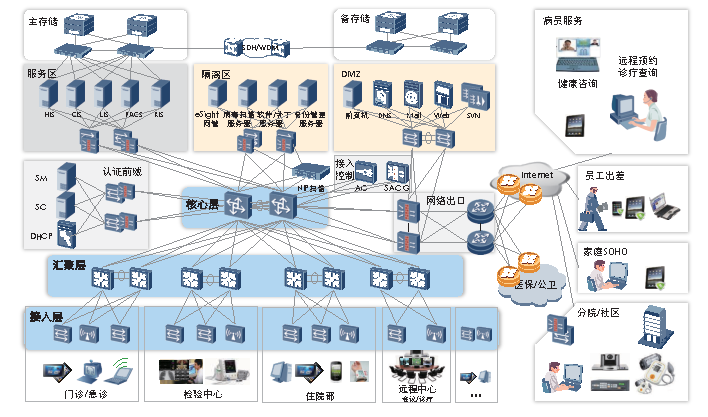
\includegraphics[width=0.8\textwidth]{figures/network.pdf}
\caption{智慧医院网络和安全解决方案图 \label{fig:networkscheme}}
\end{figure}

\section{安全策略的设计}
\label{sec:org7230e4e}

\section{物联网信息平台}
\label{sec:org6d0c8b4}

以医院信息系统为核心,将医院所有设施纳入物联网管理平台,见图\ref{fig:internetofthings}

\begin{figure}[htbp]
\centering
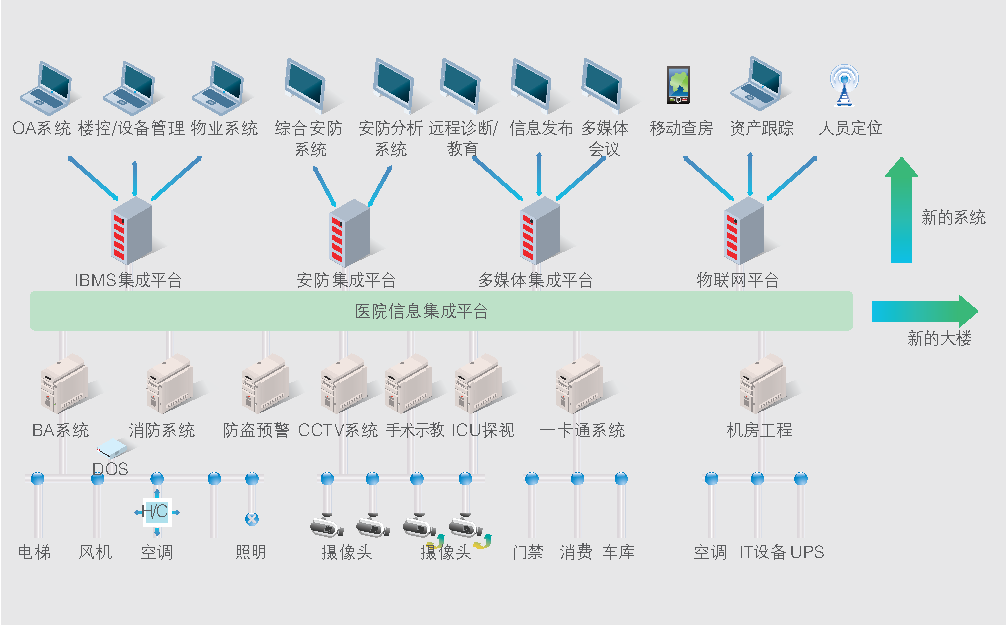
\includegraphics[width=0.8\textwidth]{figures/internetofthings.pdf}
\caption{物联网体系结构 \label{fig:internetofthings}}
\end{figure}

\chapter{智慧医院的实现}
\label{sec:orgdc3fb34}
\chapter{总结与展望}
\label{sec:orgb312cb6}
\section{总结}
\label{sec:orge2b645c}
本文主要应用信息技术对医院业务系统进行了研究,设计了方便就诊者挂号就医、查询医疗信息、在线缴费以及电子病历系统,为医院信息化提供了一整套的信息化解决方案,此系统的实施节约了大量的人力物力,并提高了工作效率。
\section{展望}
\label{sec:org71c8d84}
本论文提供的智慧医院的解决方案,在应用中也存在如下一些问题:
首先,用户使用门槛较高,大部分患者用户不能熟练的使用智能设备进行 APP 的下载和安装,进而无法享受到 APP 所带来的便利。绝大部分 APP 需要患者提供大量身份信息进行验证与绑定,这也进一步限制了患者安装使用的主动性 \cite{__2013}。

其次,用户使用活跃度较低,与大型三甲医院平均每日超过万人的挂号量相比,使用智慧医院系统进行挂号预约的用户比例仍然较低,这与用户使用习惯的培养有一定关系。同时,绝大部分患者使用 APP 只是为了一次挂号,使用频率较低,用户粘性不足。

最后,缺乏行业统一标准及政策引导。由于国内个人数字健康档案建设刚刚起步,医院间和厂商间存在“信息孤岛”的现象,进一步制约了智慧医院的普及与推广。下一步,如何联通信息孤岛将是智慧医院建设者急需解决的首要问题。

未来国内智慧医院的发展趋势必将是“更简便、更深入、更广泛”。利用信息技术手段不断降低用户使用的门槛,提供更加便捷更顺畅的就诊体验;“智慧”元素将深入到医院内外全部诊疗流程中以及居民日常健康管理中,提供全方位保障;医院与医院之间,区域与区域之间医疗合作将更加紧密,统一的智慧医院标准得到更加广泛的普及 \cite{_nfc_2016}。

由于开发时间较短、个人能力有限等原因,系统存在一些不足, 功能方面也需要进一步拓展增加,具体有以下几点 \cite{2016c}:
(1)平台功能需要进一步增加,还有许多部门可以整合到系统中,如住院部、化验 部等,更好的掌握医院信息从而更好的进行管理。此外,根据物联网“物—物”相连的定义, 下一步可以把更多的设备接入系统,如增加摄像头来实现视频监控,接入一些医疗设备, 实时方便的查看病人身体情况等 \cite{RN85}。
(2)Android 客户端的功能可继续拓展,如可查看各门诊、化验室的实时排队信息, 增加地图引导功能等 \cite{RN140}。
(3)未在系统中融合现在流行的医院一卡通系统 \cite{__2013}。
(4)本系统目前是在局域网内进行通信的,网络需要进一步拓展,真正实现随时随 地的使用 \cite{adame_cuidats:_nodate}。

%%% 其它部分
\backmatter

\bibliographystyle{plain}
\bibliography{Medicalinformation,phd,ResourcesMatching}


%% 致谢
\include{data/ack}

%% 附录
%%\begin{appendix}
%%\input{data/appendix01}
%%\end{appendix}

%% 个人简历
%%\include{data/resume}

%% 本科生进行格式审查是需要下面这个表格,答辩可能不需要。选择性留下。
% 综合论文训练记录表
%% 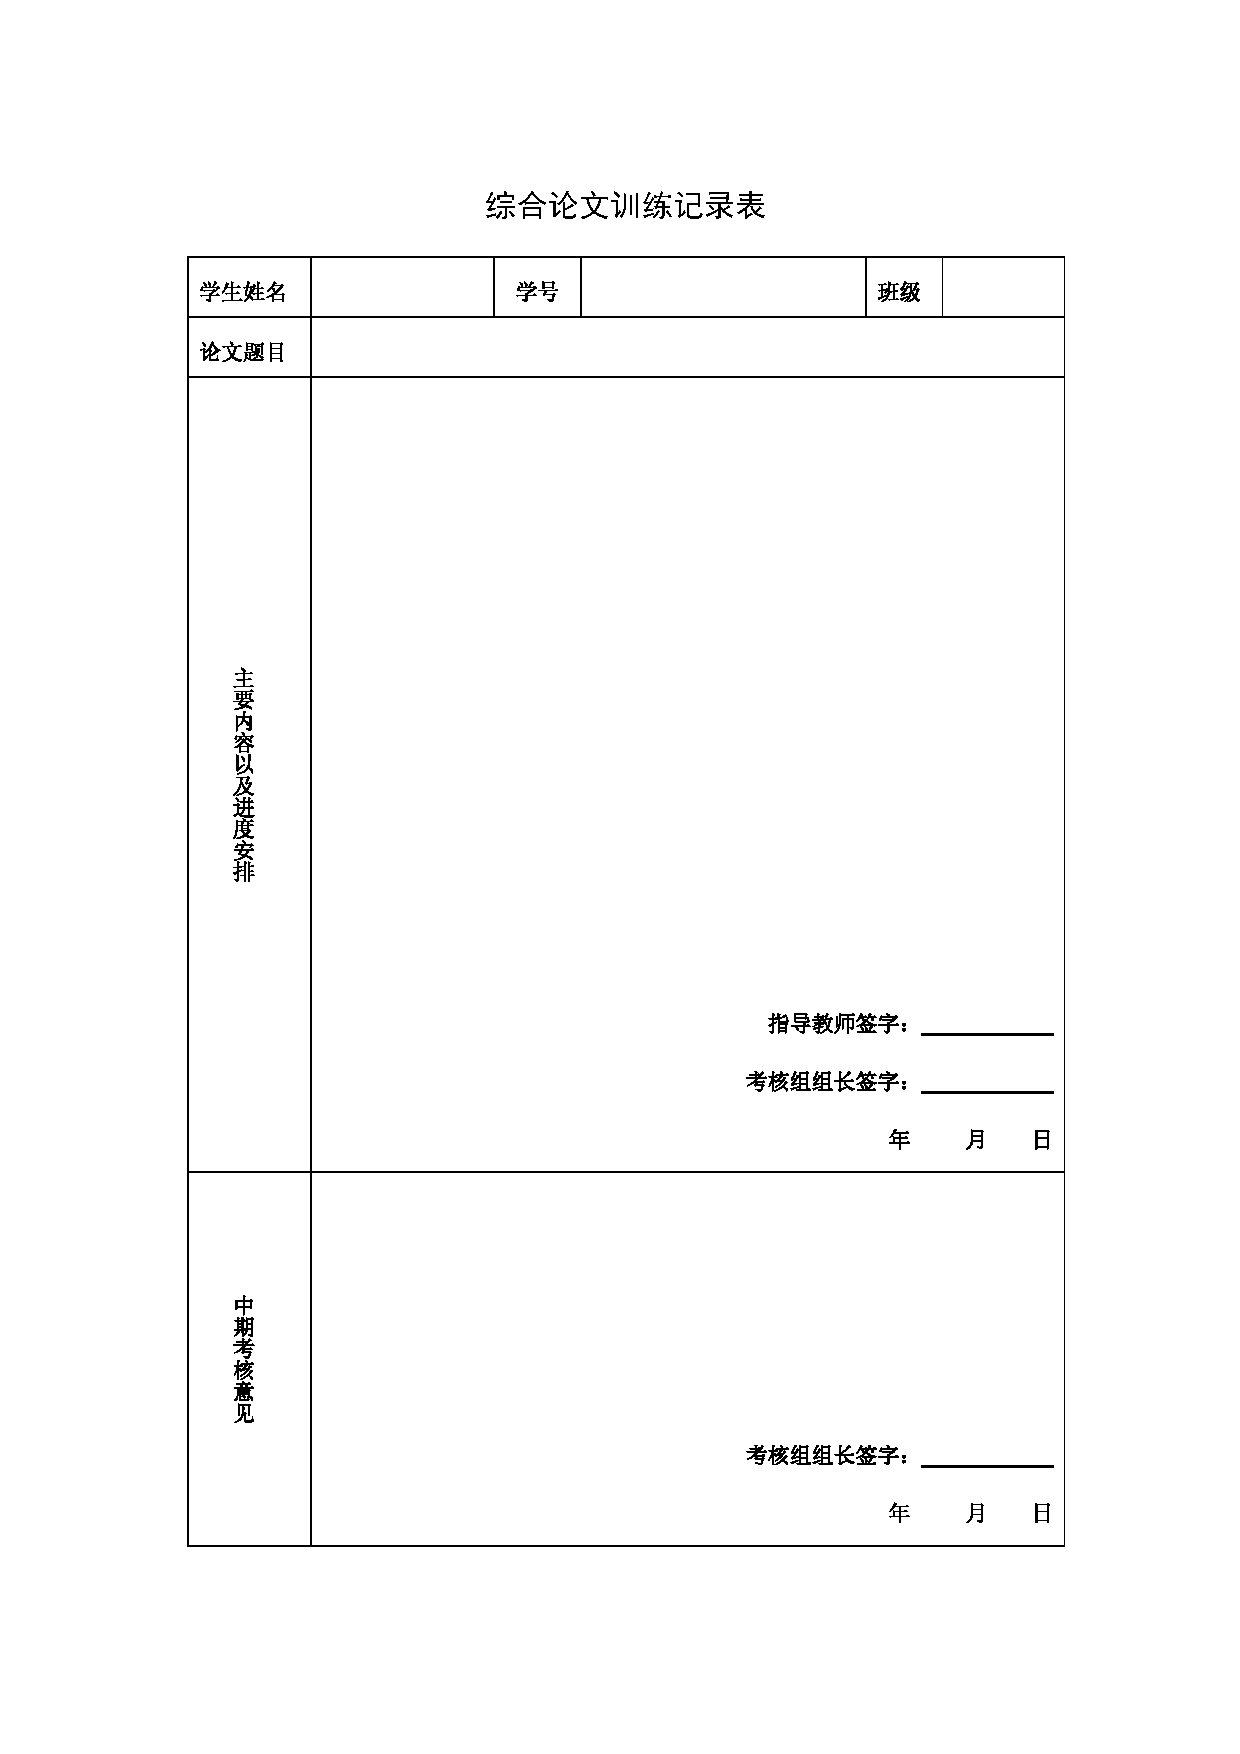
\includepdf[pages=-]{scan-record.pdf}
\end{document}